\documentclass[a4paper, 12pt, addpoints]{exam}
\usepackage[usenames,dvipsnames]{xcolor}
\usepackage{fullpage}
\usepackage[top=0.5in, bottom=1in, left=1in, right=1in]{geometry}
\usepackage{amsmath}
\usepackage{pgfornament}
\usepackage{multicol}
\usepackage{enumitem}
\usepackage{xspace}
\usepackage{lastpage}
\usepackage{hyperref}
\usepackage{tikz}
\usepackage{tkz-euclide}
\usepackage{pgfplots}
\usepackage{commath}
\usepackage{graphicx}
\usetkzobj{all}
\usepackage{lastpage}
\usetikzlibrary{shapes.misc, angles, quotes}

\pagestyle{headandfoot}
\firstpageheader{\makebox[9.5cm]{NAME \hrulefill}~\makebox[4cm]{ID \hrulefill}~\makebox[3.5cm]{Seat No.\hrulefill}}{}{}
\firstpagefooter{}{Page \thepage\ of \numpages}{}
\firstpageheadrule
\runningheader{\class~ Midterm Exam}{}{\makebox[5cm]{NAME \hrulefill}\makebox[4cm]{ID \hrulefill}}
\runningheadrule
\runningfooter{}{ Page \thepage\ of \numpages}{}

%opening

\newcommand{\epv}[1]{\ensuremath{\left< #1 \right>}\xspace}
\newcommand{\variance}{\ensuremath{\text{Var}}}
\newcommand{\unit}[1]{\;\ensuremath{\mathrm{#1}}\xspace}
\newcommand{\umss}{\;\unit{m/s^2}}
\newcommand{\ums}{\;\unit{m/s}}
\newcommand{\us}{\;\unit{s}}
\newcommand{\um}{\;\unit{m}}
\newcommand{\kwd}[1]{\textbf{\textcolor{Brown}{#1}}}
\cfoot{\pgfornament[height=1em, ydelta=-0.4em]{11} \thepage of \pageref{LastPage}  \;\pgfornament[height=1em, ydelta=-0.4em]{14}}
\newenvironment{question}{\begin{minipage}{\linewidth}}{\end{minipage}}
\rhead{Name: \underline{\hspace{7cm}} }
\lhead{ID: \underline{\hspace{4cm}} }
\headheight 15pt              %% put this outside
\headsep 10pt                 %% put this outside
\newcommand{\sanswer}{\vspace{1.25in}}
\newcommand{\manswer}{\vspace{2.5in}}
\newcommand{\lanswer}{\vspace{5in}}
\newcommand{\ssanswer}{\vspace{0.5in}}
\newcommand{\ihat}{\hat{i}}
\newcommand{\jhat}{\hat{j}}
\newcommand{\khat}{\hat{k}}
\newcommand{\hint}{\textbf{Hint:} }
\newcommand\NoIndent[1]{%
	\begingroup
	\par
	\parshape0
	#1\par
	\endgroup
}

\pgfplotsset{
	answeraxis/.style={width=6in, height = 3in, grid=both, axis lines=middle, minor tick num=1,  axis line style={very thick, gray!50!white}}
}

\begin{document}
\begin{center}
	\textcolor{orange}{\textsc{Discrete Mathematics}}\\
	\huge\textbf{\textsc{Midterm Exam T3 2021}}\\
	\pgfornament[width=0.7\textwidth, color=white!30!black]{89}
\end{center}

\textbf{Instruction}
\begin{itemize}
\item Write your name
\item Read the questions carefully.
\item This exam is open book, open notes and open internet. You are however not allowed to get help from other human being on exam via any means. (Ex: Talking to a cat for moral support is allowed.)
\item Upload the PDF on canvas by the deadline specified on canvas.
\item There are 6 problems. Each problem worths 100 points. 600 points in total. You only need to get 540 points to get full score.
\item Attempt all problems, state your reasons \emph{clearly} and \emph{legibly}, because partial credits will be given.
\end{itemize}
\vspace{0.25in}

	\begin{center}
		\def\arraystretch{1.5}
		\begin{tabular}{|c|c|c|}
			\hline Question & Full Score & Your Score  \\ 
			\hline  1 & 100 &  \\ 
			\hline  2 & 100 &  \\ 
			\hline  3 & 100 &  \\
			\hline  4 & 100 &  \\
			\hline  5 & 100 &  \\
			\hline  6 & 100 &  \\
			\hline 
		\end{tabular} 
	\end{center}
	
%\begin{center}
%	\textbf{Good luck!}  
%\end{center}
%\noindent \rule{\textwidth}{1pt}
%FOR INSTRUCTOR USED
%\begin{center}
%	\textbf{Distribution of Marks}\\
%	\medskip
%	%\gradetable[h][questions]
%\end{center}
%\medskip
%	\def\arraystretch{1.0}

%\

\begin{center}
Total:\; \fbox{ \begin{minipage}{1in} \hfill\vspace{1in} \end{minipage} }/540
\end{center}
\pagebreak
\section*{Useful Formula and Definitions}
\subsection*{Asymptotics}
\renewcommand{\arraystretch}{2}
\begin{center}
	\begin{tabular}{c |c c c | c}
		\hline\hline
		Definiton & Definition & & & Intuition\\
		\hline\hline  Asym. Equal & $f \sim g$ & iff & $\lim\limits_{x\to \infty} \frac{f(x)}{g(x)} = 1$  & $f \underbrace{\equiv}_{x \to \infty} g$\\ 
		Big Oh & $f \in O(g)$ & iff & $\lim\limits_{x\to \infty} \frac{f(x)}{g(x)} < \infty$ & $f \underbrace{\le}_{x \to \infty} g$  \\ 
		Little Oh  & $f \in o(g)$ & iff & $\lim\limits_{x\to \infty} \frac{f(x)}{g(x)} = 0$ & $f \underbrace{<}_{x \to \infty} g$ \\ 
		Little Omega & $f \in \omega(g)$ & iff & $\lim\limits_{x\to \infty} \frac{f(x)}{g(x)} \to \infty$ & $f \underbrace{>}_{x \to \infty} g$ \\ 
		Big Omega  & $f \in \Omega(g)$ & iff & $\lim\limits_{x\to \infty} \frac{f(x)}{g(x)} > 0 $ & $f \underbrace{\ge}_{x \to \infty} g$ \\ 
		Theta & $f \in \Theta(g)$ & iff & $\lim\limits_{x\to \infty} \frac{f(x)}{g(x)} =c, c\ne 0$ & $f \underbrace{=}_{x \to \infty} g$ \\ 
		\hline\hline 
	\end{tabular}
\end{center}
\subsection*{Sum}
\begin{align*}
	1 + 2 + 3 + \ldots + n &= \frac{n(n+1)}{2}\\
	1^2 + 2^2 + 3^2 + \ldots + n^2 &= \frac{n(n+1)(2n+1)}{6}\\
	1^3 + 2^3 + 3^3 + \ldots + n^3 &= \left(\frac{n(n+1)}{2}\right)^2
\end{align*}
\subsection*{Integral}
\begin{align*}
	\int x^n \; dx &= \frac{1}{n+1} x^{n+1} &\text{if } n \ne -1\\
	\int \frac{1}{x} \; dx &= \ln (x)
\end{align*}

\subsection*{Quadratic}
\begin{align*}
	x = \frac{-b \pm \sqrt{b^2 - 4ac}}{2a}
\end{align*}

\pagebreak

\begin{enumerate}
	\setlength\itemsep{1em}
	\item Easy stuff(100 points. 20 each.)
	
	\begin{enumerate}
		\item Draw truth table for 
		\[ (P \to \sim R) \land (P \lor R) \]
			\manswer
			
		
		\item Asymptotic Behavior. $f(x) = x^3 + 3x^2 + 1$, $g(x) = 2x^3$. Indicate whether the following statements are true or false.
		\begin{enumerate}
			\item  $f \in \Theta(g)$ 
			\ssanswer
			
			\item $f \in O(g)$
			\ssanswer

		\end{enumerate}

		\item Find the closed form formula for the following sum:
		\[ \sum_{i=0}^n (x^i + 5y^{i+1}) \]
		where $x, y$ are constants.
		\manswer
		\newpage
		\item Disprove the following theorem.
		\begin{center}
			$x^2 > x$ for all $x$ in positive integer.
		\end{center}
		\manswer
		\item Use integral bound to find the \emph{lowerbound} for the following sum.\[
			\sum^n_{x=1} \frac{1}{x^3}
		\]\manswer
	\end{enumerate}
	\newpage
	
	\item Easy Proof
	\begin{enumerate}
		\item (50 points)
		For any $a, b \in I$,  $a^2b + ab^2$ is always even.
		\manswer
		
		\item (50 points)
		Show that If $a|b$ and $b|c$ then $a|c$.
		
		Ex: a=3 b=54 c=108. 54 is divisible by 3 and 108 is divisible by 54 then 3 divides 108
		\manswer
		

	\end{enumerate}
	
	\newpage
	\newcommand{\ff}[1]{\left(1-\frac{1}{#1}\right)}
	\item (100 points) Show that $\forall n \ge 2$
	$$
	\ff{2}\ff{3}\ff{4}\ldots\ff{n} =  \frac{1}{n}
	$$
	
	\newpage
	\item Any n-gon(loose definition is a closed shape with n corners) can be triangulate into n-2 triangles.
	
	Ex: The figure below shows a 7-gon triangulated in to 5 triangles and a 12-gon triangulated into 10 triangles.
	
	% TODO: \usepackage{graphicx} required
	\begin{center}
		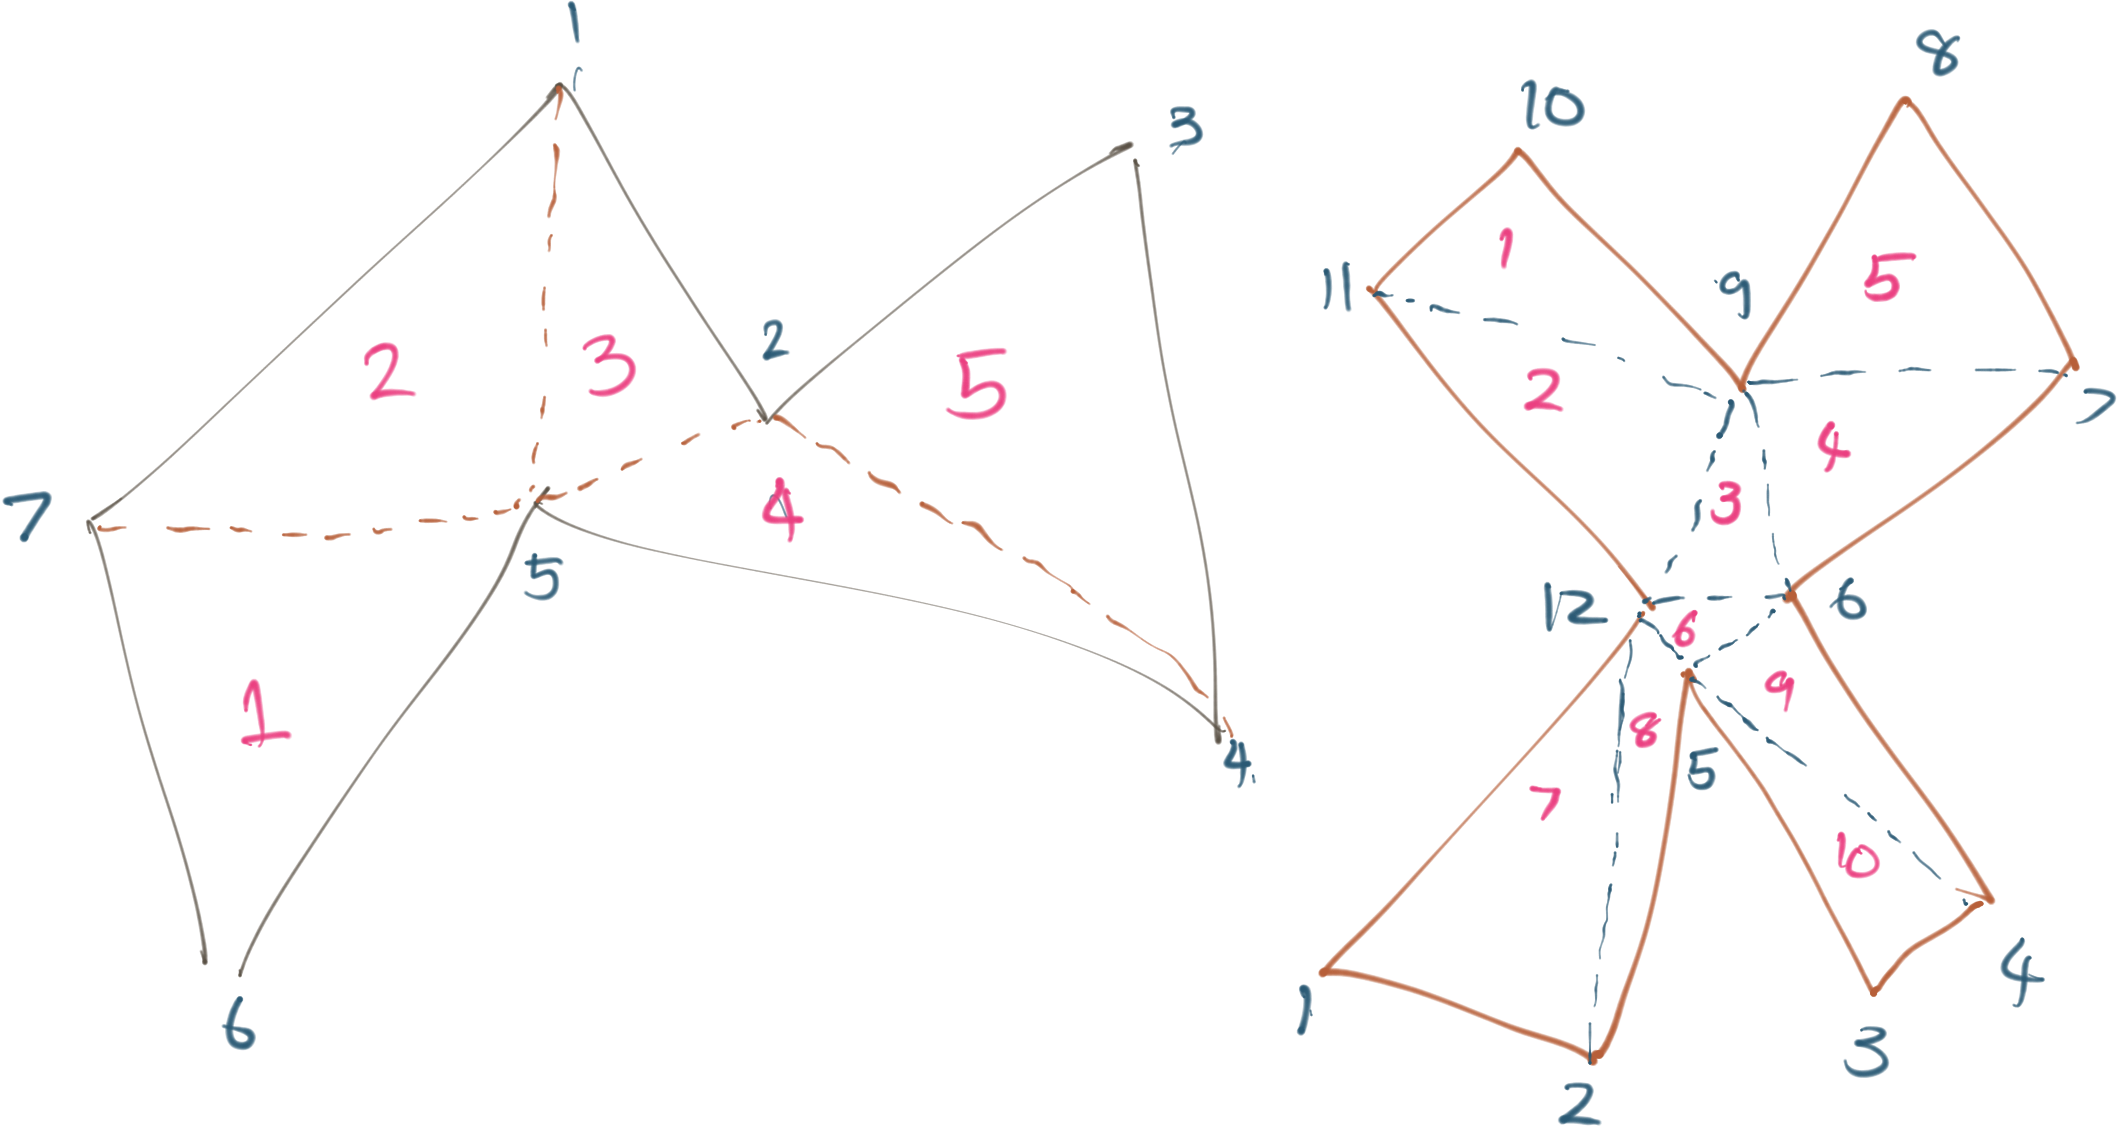
\includegraphics[width=0.7\linewidth]{n-gon}
	\end{center}
	
	
	
	

	
		
	\newpage
	\item (100 points)
	Consider a $2 \times 2$ black and white board show below.
	
	\begin{center}
			
\begin{tikzpicture}
			\draw[fill=black] (0, 0) rectangle (1, 1);
			\draw[fill=white] (0, 1) rectangle (1, 2);
			\draw[fill=white] (1, 0) rectangle (2, 1);
			\draw[fill=black] (1, 1) rectangle (2, 2);
		\end{tikzpicture}
	\end{center}
	
	Each turn you can pick a \textbf{side}(left, right, top, bottom) then flip color of the two squares on that side. Ex: if you pick left then the two squares on the left will be flipped.
	
	Show that no matter what sequence of move you choose, you can't get it to have exactly 1 white square left.
	
	\newpage
	\item (100 points)Solve the following recurrence. Just find the solution. No need to prove it using induction.:
	\begin{enumerate}
		\item (30 points)$T(n) = T(n-1) + n; T(1)=2$
		\vspace{4in}
		\item (30 points)$\displaystyle T(n)= 3T\left(\frac{n}{2}\right) + 3; T(1) = 3$
		\manswer
		\newpage
		\item (40 points)$T(n) = 18 T(n-1) - 77 T(n-2); T(0)=5, T(1)=47$
	\end{enumerate}

\end{enumerate}


\end{document}